\documentclass[11pt]{article}

% ---------- Packages ----------
\usepackage[letterpaper, margin=0.75in]{geometry}
\usepackage[T1]{fontenc}
\usepackage{mathptmx}
\usepackage{microtype}
\usepackage{tabularx}
\usepackage{booktabs}
\usepackage{array}
\usepackage{enumitem}
\usepackage{titlesec}
\usepackage[hidelinks]{hyperref}
\usepackage{xurl}
\usepackage{amsmath}
\usepackage{tikz}
\usetikzlibrary{positioning, arrows.meta, fit, backgrounds}

% ---------- Compact layout ----------
\setlength{\parindent}{0pt}
\setlength{\parskip}{2.5pt}
\titlespacing*{\section}{0pt}{6pt}{2pt}
\titleformat{\section}{\large\bfseries}{\thesection.}{0.5em}{}
\setlist{nosep, leftmargin=1.2em, topsep=1pt}
\renewcommand{\arraystretch}{1.12}
\newcolumntype{Y}{>{\raggedright\arraybackslash}X}
\newcommand{\ph}[1]{\textit{[#1]}} % placeholder text for the team to fill in

\begin{document}

% ---------- Title ----------
\begin{center}
  {\Large\bfseries LiftLens: AI Workout Planning with Video-Based Form Review}\\[2pt]
  {\large Phase 2 -- Prototype Progress Report}\\[2pt]
  Jose Fuentes \quad$\cdot$\quad Perry Wang \quad$\cdot$\quad November 2026\\[1pt]
  Repository: \url{https://github.com/fuentesjm/liftlens}
\end{center}
\vspace{-6pt}

% =====================================================
\section{Objective and Current Scope}
\textbf{Objective:} give beginner lifters the two things a trainer provides: per-rep \textbf{form feedback} from a phone video, and \textbf{progression decisions} for the next session based on that feedback.
\textbf{Current scope (MVP):} one exercise (the squat), filmed from the side and uploaded as a video. The working end-to-end flow is:
create a weekly plan $\rightarrow$ record and upload a set $\rightarrow$ per-rep report with chart, replay, and coaching notes $\rightarrow$ next set's load and reps adjusted automatically $\rightarrow$ history.

% =====================================================
\section{Completed Features and Remaining Tasks}
\vspace{-2pt}
\begin{tabularx}{\linewidth}{@{}p{0.27\linewidth}Y@{}}
\toprule
\textbf{Completed} & \textbf{What it does} \\
\midrule
Squat analysis pipeline & Pose estimation on every frame; rep segmentation; rack setup movements filtered out; camera-angle-robust depth check and forward-lean check; form score, cues, and warnings (low visibility, camera not side-on, unsteady tracking). \\
Adaptation engine & Rule-based double progression: progress, hold, reduce, deload, or retest, each with a plain-language reason. \\
LLM features & Coaching feedback and weekly plan generation with Gemini; plans checked against safety limits; template fallback. \\
FastAPI backend & Upload with validation, saved sessions, next-workout and plan endpoints; videos deleted after analysis. \\
Next.js frontend & Today, Record a set (upload progress), Results (depth chart, per-rep verdicts, synced replay), Plan, History. \\
Evaluation, tests, docs & Evaluation script on 3 labeled team clips; 150 automated tests (no video, model, or key needed); README; LLM documentation (\texttt{docs/llm.md}). \\
\midrule
\textbf{Planned (remaining)} & \textbf{Description} \\
\midrule
Larger evaluation & More lifters and held-out clips (thresholds were tuned on the current 3); a clip with clear forward lean. \\
Push-up analysis & Second exercise: depth and body-line rules. \\
Replay overlay & Draw the pose skeleton on the replay video. \\
Accounts and usability & User accounts (one shared history today); SUS usability test with beginners. \\
\bottomrule
\end{tabularx}

% =====================================================
\section{System Architecture and Workflow}
\vspace{-4pt}
\begin{center}
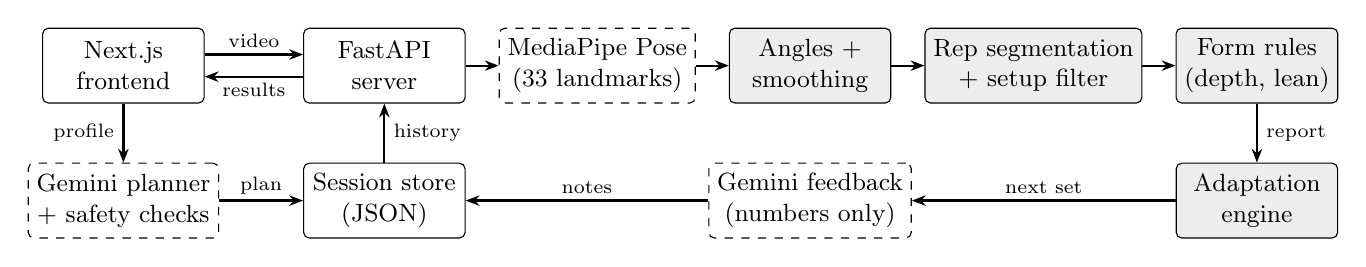
\begin{tikzpicture}[
  font=\small,
  box/.style={draw, rounded corners=2pt, align=center, inner sep=3pt, minimum height=0.95cm, minimum width=2.05cm},
  ours/.style={box, fill=gray!14},
  ext/.style={box, dashed},
  arr/.style={-{Stealth[length=5pt]}, thick},
  lab/.style={font=\scriptsize, fill=white, inner sep=1pt},
  node distance=0.75cm and 0.42cm]
  % Row 1: upload and analysis
  \node[box] (web) {Next.js\\frontend};
  \node[box, right=1.25cm of web] (api) {FastAPI\\server};
  \node[ext, right=of api] (pose) {MediaPipe Pose\\(33 landmarks)};
  \node[ours, right=of pose] (ang) {Angles +\\smoothing};
  \node[ours, right=of ang] (reps) {Rep segmentation\\+ setup filter};
  \node[ours, right=of reps] (rules) {Form rules\\(depth, lean)};
  % Row 2: decision, feedback, storage, planning
  \node[box, below=of api] (store) {Session store\\(JSON)};
  \node[ext, below=of web] (plan) {Gemini planner\\+ safety checks};
  \node[ext, below=of ang] (fb) {Gemini feedback\\(numbers only)};
  \node[ours, below=of rules] (adapt) {Adaptation\\engine};
  % Arrows
  \draw[arr] ([yshift=4pt]web.east) -- node[lab, above=1pt]{video} ([yshift=4pt]api.west);
  \draw[arr] ([yshift=-4pt]api.west) -- node[lab, below=1pt]{results} ([yshift=-4pt]web.east);
  \draw[arr] (api) -- (pose);
  \draw[arr] (pose) -- (ang);
  \draw[arr] (ang) -- (reps);
  \draw[arr] (reps) -- (rules);
  \draw[arr] (rules) -- node[lab, right=2pt]{report} (adapt);
  \draw[arr] (adapt) -- node[lab, above=1pt]{next set} (fb);
  \draw[arr] (fb) -- node[lab, above=1pt]{notes} (store);
  \draw[arr] (store) -- node[lab, right=2pt]{history} (api);
  \draw[arr] (web) -- node[lab, left=2pt]{profile} (plan);
  \draw[arr] (plan) -- node[lab, above=1pt]{plan} (store);
\end{tikzpicture}
\end{center}
\vspace{-4pt}
{\small Shaded: team-built algorithms. Dashed: pretrained model or external API. The uploaded video exists only in a temporary folder during analysis; only measurements are stored.}

% =====================================================
\section{Data and Models/Algorithms}
\begin{itemize}
  \item \textbf{Pose model (pretrained):} MediaPipe Pose Landmarker (full), run offline on every frame of the uploaded video.
  \item \textbf{Team algorithms:} gap interpolation and centered smoothing; a two-threshold rep state machine on the knee angle whose thresholds \textbf{adapt to each person's standing angle}; a \textbf{setup filter} that drops knee bends where the hands are near or above the head (ducking under a racked bar); a \textbf{camera-angle-robust depth measure}: the thigh angle above parallel from heights only, $\sin\theta = (y_\text{knee} - y_\text{hip}) / L_\text{thigh}$, with $L_\text{thigh}$ measured while standing (rotating the camera around the lifter changes horizontal distances, not heights); depth rule $\theta \le 15^\circ$ at the deepest point; lean rule ($\le 50^\circ$ from vertical); camera-angle and unsteady-tracking warnings.
  \item \textbf{Adaptation engine:} double progression within 8--12 reps (5\,lb / 2.5\,kg steps), hold for form score 0.5--0.8 or RPE 9--10, reduce on missed reps or poor form, deload after two poor sessions.
  \item \textbf{External LLM (Gemini \texttt{gemini-3.5-flash-lite}, JSON mode):} rewrites results as coaching text and proposes weekly plans. Only numbers, error codes, and a structured profile are sent. Our code validates every reply, enforces plan safety limits (exercise list, sets, reps, rest, daily cap), retries once with the violations listed, and falls back to templates. Prompts, input/output examples, and limitations are in \texttt{docs/llm.md}; credentials are read from a gitignored \texttt{.env} file.
  \item \textbf{Data:} 3 side-view squat clips of one team member, recorded by Perry Wang (empty bar with good form, loaded bar with good form, shallow reps), labeled with true rep counts and faulty reps; synthetic squat sequences with known geometry for automated tests.
  \item \textbf{Change from Phase 1:} analysis runs on a Python server instead of in the browser. It was faster to build and test, and the privacy goal is kept by deleting each video right after analysis.
\end{itemize}

% =====================================================
\section{Preliminary Results}
Evaluation with \texttt{scripts/evaluate.py} on the 3 labeled clips (output in \texttt{docs/eval\_results.json}):

\vspace{-2pt}
\begin{tabularx}{\linewidth}{@{}>{\raggedright\arraybackslash}p{0.24\linewidth}>{\raggedright\arraybackslash}p{0.14\linewidth}>{\raggedright\arraybackslash}p{0.2\linewidth}Y@{}}
\toprule
\textbf{Clip} & \textbf{Reps (true / found)} & \textbf{Shallow reps (true / flagged)} & \textbf{Notes} \\
\midrule
Empty bar, good form & 3 / 3 & none / none & Unrack and re-rack ignored \\
Loaded bar, good form & 3 / 4 & none / 1--4 & Plates and rack hide the hips; unsteady-tracking warning shown \\
Bad form (shallow) & 3 / 3 & 1--3 / 1--3 & Re-rack ignored \\
\bottomrule
\end{tabularx}

Rep count was exact on 2 of 3 clips (mean absolute error 0.33 reps per clip). Shallow-depth detection on clips with the correct count: 3 true positives, 0 false positives, 0 misses. Processing took about 0.6\,s per second of video on an Apple M1 laptop. Gemini \texttt{gemini-3.5-flash-lite} answered in 1.3\,s (feedback) and 1.7\,s (plan), valid on the first attempt; \texttt{gemini-3.8-flash} timed out (HTTP 504), so we switched models. \textbf{What the first evaluation changed:} the original version counted 4, 6, and 4 reps on these clips (unracking and re-racking counted as reps) and passed all 3 shallow reps, because the on-screen knee angle read 84--94$^\circ$ under a slightly angled camera while the thighs were 22--28$^\circ$ above parallel. This led to the setup filter and the height-based depth measure. Because the thresholds were tuned on these same clips, these numbers show feasibility, not general accuracy.

% =====================================================
\section{Known Limitations}
\begin{itemize}
  \item Small evaluation: 3 clips of one lifter, used both to tune and to test the thresholds. The lean rule has not been tested on a clip with a clear lean.
  \item Occlusion (plates, rack) breaks tracking; the app warns but cannot correct it. Squats only, side view only; the phone should be upright and level. Knee cave-in is not checked.
  \item No user accounts; replay works only right after upload because videos are not stored.
  \item Gemini's free tier may use prompts for product improvement (we send numbers only); LLM wording is not checked word by word. Decisions always come from our code. Not medical advice.
\end{itemize}

% =====================================================
\section{Team Responsibilities}
\begin{itemize}
  \item \textbf{Jose Fuentes:} backend: video analysis pipeline, adaptation engine, LLM integration, FastAPI server, automated tests, and repository documentation.
  \item \textbf{Perry Wang:} frontend: Next.js pages, upload flow, results chart and replay; recorded the team's test clips.
\end{itemize}

\end{document}
